

   \chapter{Page tables}   
    \label{CH:MEM}     

页表是最流行的机制,操作系统通过它为每个进程提供自己的私有地址空间和内存。页表确定内存地址的含义以及可以访问物理内存的哪些部分。它们允许 xv6 隔离不同进程的地址空间并将它们复用到单个物理内存上。页表是一种流行的设计,因为它们提供了一定程度的间接性,允许操作系统执行许多技巧。 Xv6 执行一些技巧:在多个地址空间中映射相同的内存( trampoline 页面),并使用未映射的页面保护内核和用户堆栈。本章的其余部分解释了 RISC-V 硬件提供的页表以及 xv6 如何使用它们。
    \section{Paging hardware}    提醒一下,RISC-V 指令(用户和内核)操作虚拟地址。机器的 RAM(或物理内存)通过物理地址进行索引。 RISC-V页表硬件通过将每个虚拟地址映射到物理地址来连接这两种地址。  

   \begin{figure}[t]
\center
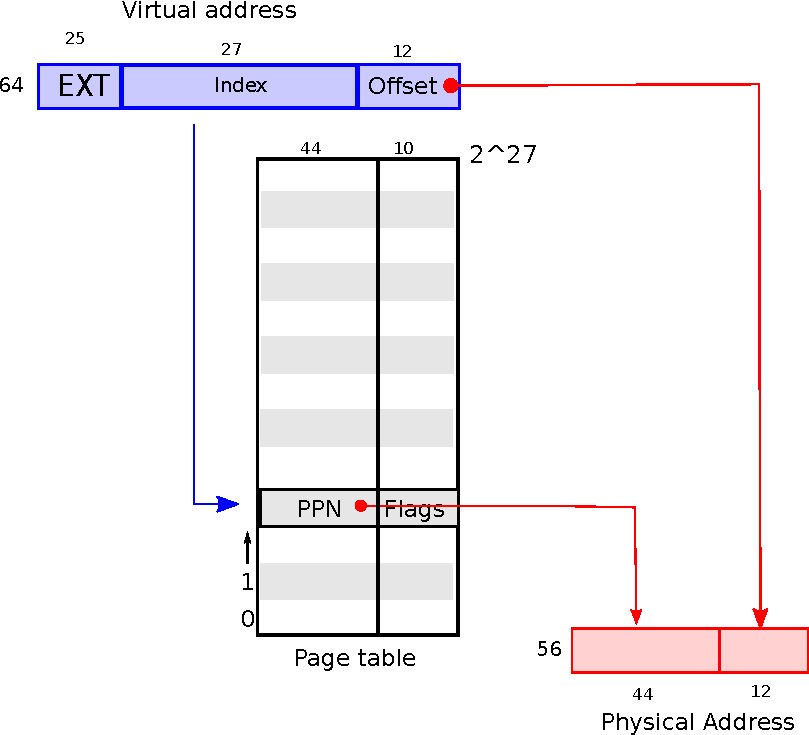
\includegraphics[scale=0.5]{fig/riscv_address.pdf}
\caption{RISC-V 虚拟和物理地址,具有简化的逻辑页表。  }
\label{fig:riscv_address}
\end{figure}     

xv6运行在Sv39 RISC-V上,这意味着只使用64位虚拟地址的底部39位;前 25 位未使用。在此 Sv39 配置中,RISC-V 页表逻辑上是    $2^{27}$    (134,217,728) 的数组
    \indextext{page table entries (PTEs)}    。每个 PTE 包含一个 44 位物理页号 (PPN) 和一些标志。分页硬件通过使用39位中的高27位索引到页表中找到PTE来翻译虚拟地址,并制作一个56位物理地址,其高44位来自PTE中的PPN,其低12位被复制来自原始虚拟地址。图~    \ref{fig:riscv_address}    通过将页表的逻辑视图显示为简单的 PTE 数组来显示此过程(有关更完整的情况,请参见图~    \ref{fig:riscv_pagetable}   )。页表使操作系统能够以 4096 (    $2^{12}$    ) 字节对齐块的粒度控制虚拟到物理地址转换。这样的块称为    \indextext{page}    。  

   \begin{figure}[t]
\center
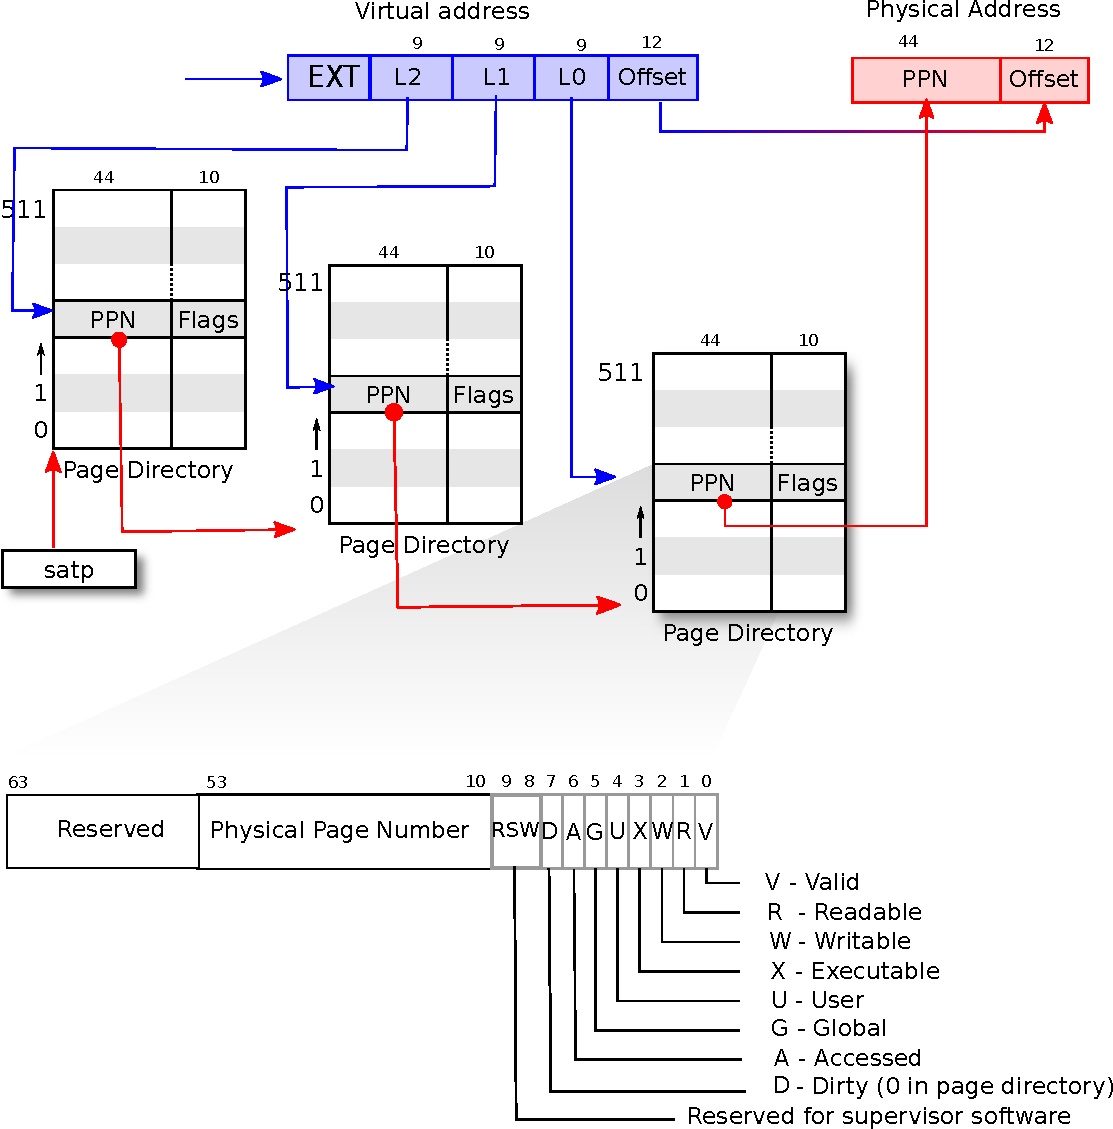
\includegraphics[scale=0.5]{fig/riscv_pagetable.pdf}
\caption{RISC-V 地址转换详细信息。  }
\label{fig:riscv_pagetable}
\end{figure}     

在 Sv39 RISC-V 中,虚拟地址的前 25 位不用于翻译。物理地址也有增长的空间:PTE 格式中有空间让物理页号再增长 10 位。 RISC-V 的设计者根据技术预测选择了这些数字。    $2^{39}$    字节为 512 GB,这对于在 RISC-V 计算机上运行的应用程序来说应该有足够的地址空间。    $2^{56}$    在不久的将来有足够的物理内存空间来容纳许多 I/O 设备和 DRAM 芯片。如果需要更多,RISC-V 设计人员已经定义了具有 48 位虚拟地址的 Sv48~    \cite{riscv:priv}    。  

如图~    \ref{fig:riscv_pagetable}    所示,RISC-V CPU 通过三个步骤将虚拟地址转换为物理地址。页表作为三层树存储在物理内存中。树的根是一个 4096 字节的页表页,包含 512 个 PTE,其中包含树的下一级页表页的物理地址。每个页面都包含树中最终级别的 512 个 PTE。分页硬件使用这 27 位中的前 9 位来选择根页表页中的 PTE,中间 9 位来选择树的下一级页表页中的 PTE,最后 9 位来选择期末PTE。 (在 Sv48 RISC-V 中,页表有四级,虚拟地址索引的位 39 到 47 位于顶层。)  

如果转换地址所需的三个 PTE 中的任何一个不存在,则分页硬件会引发    \indextext{page-fault exception}    ,将其留给内核来处理异常(请参阅第    \ref{CH:TRAP}    章)。  

与图~    \ref{fig:riscv_address}    的单层设计相比,图~    \ref{fig:riscv_pagetable}    的三层结构允许以内存高效的方式记录PTE。在大范围的虚拟地址没有映射的常见情况下,三级结构可以省略整个页目录。例如,如果应用程序仅使用从地址 0 开始的几个页,则顶级页目录的 1 到 511 项无效,并且内核不必为 511 中间页目录分配这些页。此外,内核也不必为那些 511 中间页目录的底层页目录分配页。因此,在本例中,三级设计为中间页目录保存了 511 个页面,
    $511\times512$    页面用于底层页面目录。  

尽管 CPU 在硬件中遍历三级结构作为执行加载或存储指令的一部分,但三级结构的潜在缺点是 CPU 必须从内存加载三个 PTE 来执行加载/存储指令中的虚拟地址到物理地址的转换。为了避免从物理内存加载 PTE 的成本,RISC-V CPU 将页表条目缓存在
    \indextext{Translation Look-aside Buffer (TLB)}    。  

每个 PTE 都包含标志位,这些标志位告诉分页硬件如何允许使用关联的虚拟地址。
    \indexcode{PTE_V}    指示 PTE 是否存在:如果未设置,则对该页面的引用会导致异常(即不允许)。
    \indexcode{PTE_R}    控制是否允许指令读取该页。
    \indexcode{PTE_W}    控制是否允许指令写入该页。
    \indexcode{PTE_X}    控制 CPU 是否可以将页面内容解释为指令并执行它们。
    \indexcode{PTE_U}    控制是否允许用户模式下的指令访问该页面;如果未设置    \indexcode{PTE_U}   ,则 PTE 只能在超级用户模式下使用。图~    \ref{fig:riscv_pagetable}    显示了它是如何工作的。标志和所有其他页面硬件相关的结构定义在
    \fileref{kernel/riscv.h}     

为了告诉CPU使用页表,内核必须将根页表页的物理地址写入
    \texttt{satp}       \index{satp@\lstinline{satp}}    寄存器。 CPU 将使用其自己的    \texttt{satp}    指向的页表来转换后续指令生成的所有地址。每个CPU都有自己的   \texttt{satp}   ,以便不同的CPU可以运行不同的进程,每个进程都有一个由自己的页表描述的私有地址空间。  

通常,内核将所有物理内存映射到其页表中,以便它可以使用加载/存储指令读取和写入物理内存中的任何位置。由于页目录位于物理内存中,因此内核可以通过使用标准存储指令写入 PTE 的虚拟地址来对页目录中的 PTE 内容进行编程。  

关于术语的一些注释。物理内存是指DRAM中的存储单元。物理内存的一个字节有一个地址,称为物理地址。指令仅使用虚拟地址,分页硬件将其转换为物理地址,然后发送到 DRAM 硬件以读取或写入存储。与物理内存和虚拟地址不同,虚拟内存不是物理对象,而是指内核提供的用于管理物理内存和虚拟地址的抽象和机制的集合。  

   \begin{figure}[h]
\centering
 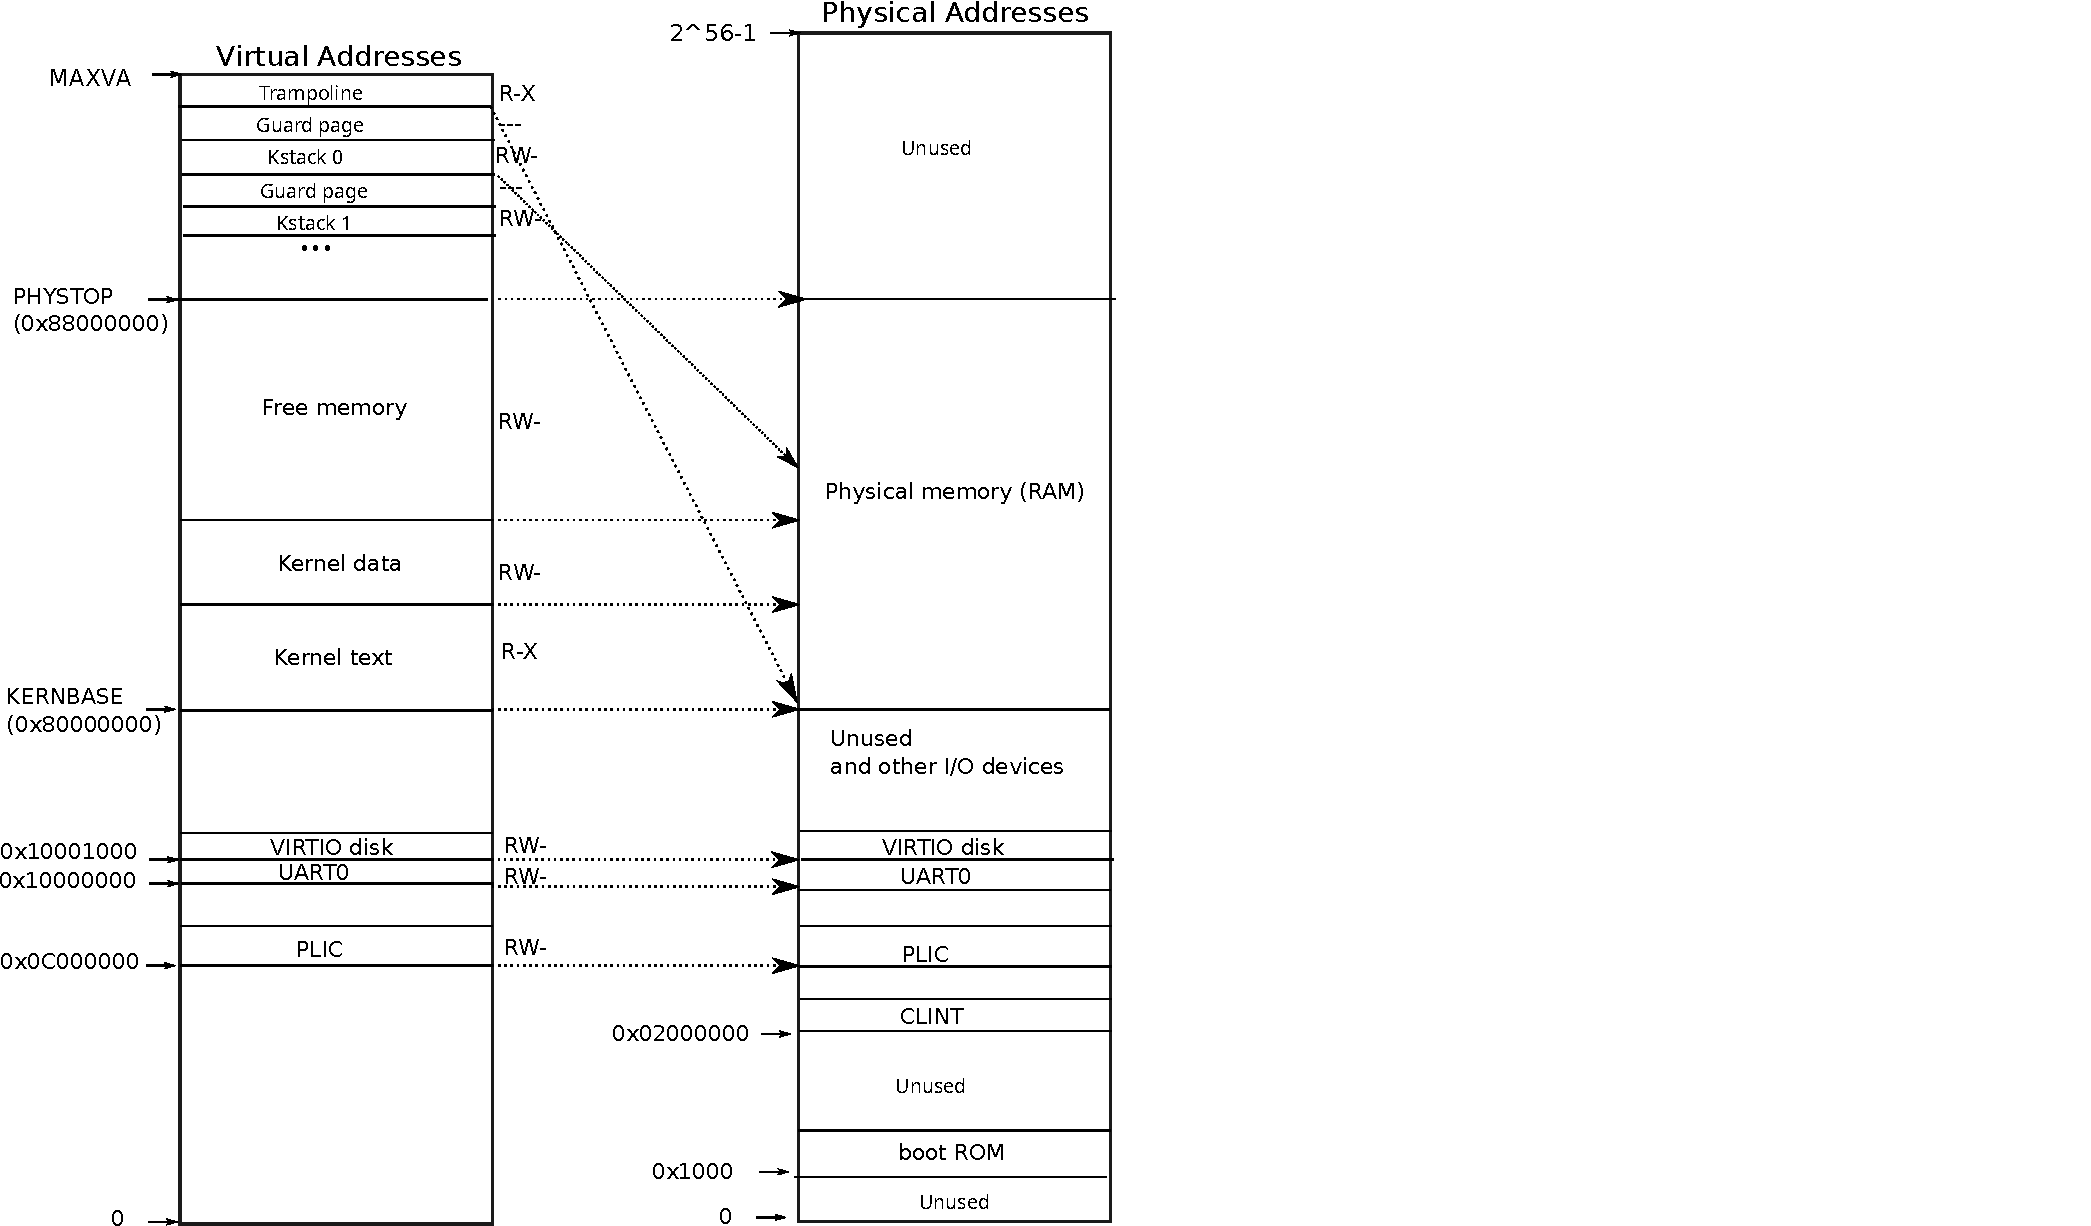
\includegraphics[scale=0.65]{fig/xv6_layout.pdf}
\caption{左边是 xv6 的内核地址空间。
  {    \sf       \small{RWX}      }  指 PTE 读、写和执行权限。右侧是 xv6 期望看到的 RISC-V 物理地址空间。  }
\label{fig:xv6_layout}
\end{figure}   
    \section{内核地址空间  }    Xv6 为每个进程维护一个页表,描述每个进程的用户地址空间,以及一个描述内核地址空间的页表。内核配置其地址空间的布局,以使其能够访问可预测虚拟地址的物理内存和各种硬件资源。图~    \ref{fig:xv6_layout}    显示了此布局如何将内核虚拟地址映射到物理地址。文件
    \fileref{kernel/memlayout.h}    声明 xv6 内核内存布局的常量。  

QEMU 模拟一台包含 RAM(物理内存)的计算机,该 RAM 从物理地址    \texttt{0x80000000}    开始,并至少持续到    \texttt{0x88000000}    ,xv6 称之为    \texttt{PHYSTOP}    。 QEMU 模拟还包括 I/O 设备,例如磁盘接口。 QEMU 将设备接口公开给软件:
    \indextext{memory-mapped}    控制寄存器位于下面
 物理地址空间中的    \texttt{0x80000000}   。内核可以通过读/写这些特殊的物理地址来与设备进行交互;此类读取和写入与设备硬件而不是 RAM 进行通信。 Chapter~    \ref{CH:TRAP}    解释展示 xv6 与设备的交互。  

内核使用“直接映射”获取 RAM 和内存映射设备寄存器;即将资源映射到等于物理地址的虚拟地址。例如,内核本身在虚拟地址空间和物理内存中都位于    \lstinline{KERNBASE=0x80000000}   。直接映射简化了读取或写入物理内存的内核代码。例如,当   \lstinline{fork}   为子进程分配用户内存时,分配器返回该内存的物理地址;
    \lstinline{fork}    在将父进程的用户内存复制到子进程时直接使用该地址作为虚拟地址。  

有几个未直接映射的内核虚拟地址:  

   \begin{itemize}

 
   \item   trampoline 页。它映射在虚拟地址空间的顶部;用户页表具有相同的映射。 Chapter~    \ref{CH:TRAP}    讨论了 trampoline 页的作用,但我们在这里看到了页表的一个有趣的用例;物理页(保存 trampoline 代码)在内核的虚拟地址空间中映射两次:一次在虚拟地址空间的顶部,一次是直接映射。   \item   内核堆栈页。每个进程都有自己的内核堆栈,该堆栈被映射到高位,以便在其下方 xv6 可以留下未映射的    \indextext{guard
    page}    。保护页面的 PTE 无效(即
    \lstinline{PTE_V}    未设置),因此如果内核溢出内核堆栈,很可能会导致异常并且内核会出现Panic。如果没有保护页,溢出的堆栈将覆盖其他内核内存,从而导致不正确的操作。Panic崩溃是更好的选择。  \end{itemize}     

虽然内核通过高内存映射使用其堆栈,但内核也可以通过直接映射地址访问它们。另一种设计可能只有直接映射,并在直接映射地址处使用堆栈。然而,在这种安排中,提供保护页将涉及取消虚拟地址的映射,否则这些虚拟地址将引用物理内存,从而难以使用。  

内核使用权限映射 trampoline 页面和内核文本
    \lstinline{PTE_R}    和
    \lstinline{PTE_X}    。内核从这些页面读取并执行指令。内核将其他页面映射到权限
    \lstinline{PTE_R}    和
    \lstinline{PTE_W}    ,以便它可以读写这些页面中的内存。保护页的映射无效。
    \section{代码:创建地址空间  }     

大多数用于操作地址空间和页表的 xv6 代码都驻留在  {    \tt    vm.c   }  中
    \lineref{kernel/vm.c:1}    。中心数据结构是  {    \tt    pagetable\_t   }  ,它实际上是指向 RISC-V 根页表页的指针; {    \tt    pagetable\_t   }  可以是内核页表,也可以是每进程页表之一。核心功能是  {    \tt    walk   }  ,它查找虚拟地址的 PTE ,以及  {    \tt    mappages   }  ,它为新映射安装 PTE 。以  {    \tt    kvm   }  开头的函数操作内核页表;以  {    \tt    uvm   }  开头的函数操作用户页表;两者都使用其他功能。
  {    \tt    copyout   }  和  {    \tt    copyin   }  将数据复制到作为系统调用参数提供的用户虚拟地址;它们位于  {    \tt    vm.c   }  中,因为它们需要显式转换这些地址才能找到相应的物理内存。  

在启动顺序的早期,
    \indexcode{main}    次调用
    \indexcode{kvminit}   
    \lineref{kernel/vm.c:/^kvminit/}    使用以下命令创建内核的页表
    \indexcode{kvmmake}   
    \lineref{kernel/vm.c:/^kvmmake/}    。此调用发生在 xv6 在 RISC-V 上启用分页之前,因此地址直接引用物理内存。
    \lstinline{kvmmake}    首先分配物理内存页来保存根页表页。然后它调用
    \indexcode{kvmmap}    安装内核所需的翻译。翻译包括内核的指令和数据、物理内存高达
    \indexcode{PHYSTOP}    和实际上是设备的内存范围。
    \indexcode{proc_mapstacks}   
    \lineref{kernel/proc.c:/^proc_mapstacks/}    为每个进程分配一个内核堆栈。它调用    \lstinline{kvmmap}    将每个堆栈映射到由
    \lstinline{KSTACK}    ,为无效的堆栈保护页留出空间。  

   \indexcode{kvmmap}   
    \lineref{kernel/vm.c:/^kvmmap/}    调用
    \indexcode{mappages}   
    \lineref{kernel/vm.c:/^mappages/}    ,它将一系列虚拟地址到相应物理地址范围的映射安装到页表中。它以页面间隔为范围内的每个虚拟地址单独执行此操作。对于每个要映射的虚拟地址,
    \lstinline{mappages}    调用
    \indexcode{walk}    查找该地址的 PTE 地址。然后它初始化 PTE 以保存相关的物理页码、所需的权限(    \lstinline{PTE_W}    、
    \lstinline{PTE_X}    和/或
    \lstinline{PTE_R}    ),以及
    \lstinline{PTE_V}    将 PTE 标记为有效
    \lineref{kernel/vm.c:/perm...PTE_V/}    。  

   \indexcode{walk}   
    \lineref{kernel/vm.c:/^walk/}    模仿 RISC-V 分页硬件,因为它在 PTE 中查找虚拟地址(见图    \ref{fig:riscv_pagetable}   )。
    \lstinline{walk}    此时将 3 级页表下降 9 位。它使用每级的 9 位虚拟地址来查找下一级页表或最终页的 PTE
    \lineref{kernel/vm.c:/pte.=..pagetable/}    。如果 PTE 无效,则所需的页面尚未分配;如果
    \lstinline{alloc}    参数已设置,
    \lstinline{walk}    分配一个新的页表页并将其物理地址放入 PTE 中。它返回树中最底层的PTE的地址
    \lineref{kernel/vm.c:/return..pagetable/}   。  

上面的代码依赖于直接映射到内核虚拟地址空间的物理内存。例如,当    \lstinline{walk}    降低页表的级别时,它会从 PTE    \lineref{kernel/vm.c:/pagetable.=..pa.*E2P/}    中提取下一级页表的(物理)地址,然后使用该地址作为虚拟地址来获取下一级的 PTE
    \lineref{kernel/vm.c:/t..pte.=..paget/}    。  

   \indexcode{main}    次调用
    \indexcode{kvminithart}   
    \lineref{kernel/vm.c:/^kvminithart/}    安装内核页表。它将根页表页的物理地址写入寄存器
    \texttt{satp}    。此后,CPU 将使用内核页表转换地址。由于内核使用恒等映射,因此下一条指令的现在虚拟地址将映射到正确的物理内存地址。  

每个 RISC-V CPU 将页表条目缓存在一个
    \indextext{Translation Look-aside Buffer (TLB)}    ,当 xv6 更改页表时,它必须告诉 CPU 使相应的缓存 TLB 条目无效。如果没有,那么在稍后的某个时刻,TLB 可能会使用旧的缓存映射,指向同时已分配给另一个进程的物理页,因此,进程可能能够在其他进程的内存上乱写乱画。 RISC-V 有一条指令    \indexcode{sfence.vma}   ,用于刷新当前 CPU 的 TLB。 Xv6重新加载后在 {    \tt    kvminithart   } 中执行 {    \tt    sfence.vma   } 
    \texttt{satp}   寄存器,以及在返回用户空间之前切换到用户页表的trampoline代码中
    \lineref{kernel/trampoline.S:/sfence.vma/}    。  

更改前还需要发出    \texttt{sfence.vma}   
    \texttt{satp}    ,以便等待所有未完成的加载和存储完成。这一等待可确保先前对页表的更新已完成,并确保先前的加载和存储使用旧页表,而不是新页表。  

为了避免刷新整个 TLB,RISC-V CPU 可能支持地址空间标识符 (ASID)~    \cite{riscv:priv}    。然后内核可以仅刷新特定地址空间的 TLB 条目。 Xv6没有使用这个功能。  

   \section{物理内存分配  }     

内核必须在运行时为页表、用户内存、内核堆栈和管道缓冲区分配和释放物理内存。  

xv6 使用内核末尾和
    \indexcode{PHYSTOP}    用于运行时分配。它一次分配和释放整个 4096 字节页面。它通过将链接列表穿过页面本身来跟踪哪些页面是空闲的。分配包括从链表中删除页面;释放包括将释放的页面添加到列表中。
    \section{代码:物理内存分配器  }     

分配器驻留在  {    \tt    kalloc.c   }     \lineref{kernel/kalloc.c:1}    中。分配器的数据结构是可用于分配的物理内存页的空闲列表。每个空闲页面的列表元素是
    \indexcode{struct run}   
    \lineref{kernel/kalloc.c:/^struct.run/}    。分配器从哪里获取内存来保存该数据结构?它存储每个免费页面的
 空闲页面本身中的    \lstinline{run}    结构,因为那里没有存储任何其他内容。空闲列表受自旋锁保护
    \linerefs{kernel/kalloc.c:/^struct.{/,/}/}    。列表和锁包装在一个结构中,以明确锁保护结构中的字段。现在,忽略锁和调用
    \lstinline{acquire}    和
    \lstinline{release}   ;第~    \ref{CH:LOCK}    章将详细研究锁定。  

功能
    \indexcode{main}    次调用
    \indexcode{kinit}    初始化分配器
    \lineref{kernel/kalloc.c:/^kinit/}    。
    \lstinline{kinit}    初始化空闲列表以保存内核末尾和  {    \tt    PHYSTOP   }  之间的每个页面。 Xv6 应该通过解析硬件提供的配置信息来确定有多少物理内存可用。相反,xv6 假设机器有 128 MB RAM。
    \lstinline{kinit}    调用
    \indexcode{freerange}    通过每页调用将内存添加到空闲列表
    \indexcode{kfree}    。 PTE 只能引用在 4096 字节边界(是 4096 的倍数)上对齐的物理地址,因此
    \lstinline{freerange}    使用
    \indexcode{PGROUNDUP}    以确保它仅释放对齐的物理地址。分配器在没有内存的情况下启动;这些调用
    \lstinline{kfree}    给它一些管理。  

分配器有时将地址视为整数,以便对它们执行算术(例如,遍历
    \lstinline{freerange}    ),有时使用地址作为读写内存的指针(例如,操纵
    \lstinline{run}    结构存储在每个页中);这种地址的双重使用是分配器代码充满 C 类型转换的主要原因。
    \index{type cast}    另一个原因是释放和分配本质上改变了内存的类型。  

功能
    \lstinline{kfree}   
    \lineref{kernel/kalloc.c:/^kfree/}    首先将要释放的内存中的每个字节设置为值 1。这将导致在释放内存后使用内存的代码(使用“悬空引用”)读取垃圾而不是旧的有效内容;希望这会导致这样的代码打破得更快。然后
    \lstinline{kfree}    将页面添加到空闲列表之前:它进行强制转换
    \lstinline{pa}    指向的指针
    \lstinline{struct}   
    \lstinline{run}    ,记录空闲列表的旧开始
    \lstinline{r->next}    ,并将空闲列表设置为
    \lstinline{r}   。
    \indexcode{kalloc}    删除并返回空闲列表中的第一个元素。  

   \section{进程地址空间  }     

每个进程都有一个单独的页表,当xv6在进程之间切换时,它也会更改页表。图~    \ref{fig:processlayout}    比图~    \ref{fig:as}    更详细地显示了进程的地址空间。进程的用户内存从虚拟地址 0 开始,可以增长到    \texttt{MAXVA}   
    \lineref{kernel/riscv.h:/MAXVA/}    ,原则上允许进程寻址 256 GB 内存。  

进程的地址空间由包含程序文本的页面组成(xv6 使用权限    \lstinline{PTE_R}    进行映射,
    \lstinline{PTE_X}    和    \lstinline{PTE_U}    ),包含程序预初始化数据的页面、堆栈页面和堆页面。 Xv6将数据、栈、堆与权限进行映射
    \lstinline{PTE_R}    、    \lstinline{PTE_W}    和    \lstinline{PTE_U}    。  

在用户地址空间内使用权限是强化用户进程的常用技术。如果文本被映射为
    \lstinline{PTE_W}    ,那么进程可能会意外修改自己的程序;例如,编程错误可能会导致程序写入空指针,修改地址 0 处的指令,然后继续运行,这可能会造成更多破坏。为了立即检测此类错误,xv6 映射不带    \lstinline{PTE_W}    的文本;如果程序意外地尝试存储到地址 0,硬件将拒绝执行存储并引发页错误(请参阅第    \ref{sec:pagefaults}    节)。然后内核终止该进程并打印出一条信息性消息,以便开发人员可以追踪问题。  

类似地,通过在没有    \lstinline{PTE_X}    的情况下映射数据,用户程序不会意外跳转到程序数据中的某个地址并在该地址开始执行。  

在现实世界中,通过仔细设置权限来强化流程也有助于防御安全攻击。对手可能会向程序(例如 Web 服务器)提供精心构造的输入,从而触发程序中的错误,希望将该错误转化为漏洞利用~    \cite{aleph:smashing}    。仔细设置权限和其他技术(例如随机化用户地址空间的布局)会使此类攻击更加困难。  

堆栈是一个单页,并显示由 exec 创建的初始内容。包含命令行参数的字符串以及指向它们的指针数组位于堆栈的最顶部。就在其下方是允许程序启动的值
    \lstinline{main}    就像函数    \lstinline{main(argc}    一样,
    \lstinline{argv)}    刚刚被调用。  

为了检测用户堆栈溢出分配的堆栈内存,xv6 通过清除    \lstinline{PTE_U}    标志在堆栈正下方放置一个不可访问的保护页。如果用户堆栈溢出并且进程尝试使用堆栈下方的地址,则硬件将生成页面错误异常,因为在用户模式下运行的程序无法访问保护页。现实世界的操作系统可能会在用户堆栈溢出时自动为其分配更多内存。  

当进程向 xv6 请求更多用户内存时,xv6 会增加进程的堆。 Xv6首先使用 {    \tt    kalloc   } 来分配物理页。然后它将 PTE 添加到指向新物理页的进程页表中。 Xv6 设置
    \lstinline{PTE_W}    ,
    \lstinline{PTE_R}    ,
    \lstinline{PTE_U}    和
 这些 PTE 中的    \lstinline{PTE_V}    标志。大多数进程不使用整个用户地址空间;xv6 离开
    \lstinline{PTE_V}    在未使用的 PTE 中清除。  

我们在这里看到一些使用页表的很好的例子。首先,不同进程的页表将用户地址转换为不同的物理内存页,从而每个进程都拥有私有的用户内存。其次,每个进程将其内存视为具有从零开始的连续虚拟地址,而进程的物理内存可以是不连续的。第三,内核用trampoline代码映射一个页面到用户地址空间的顶部(没有
    \lstinline{PTE_U}    ),因此单页物理内存显示在所有地址空间中,但只能由内核使用。  

   \begin{figure}[t]
\center
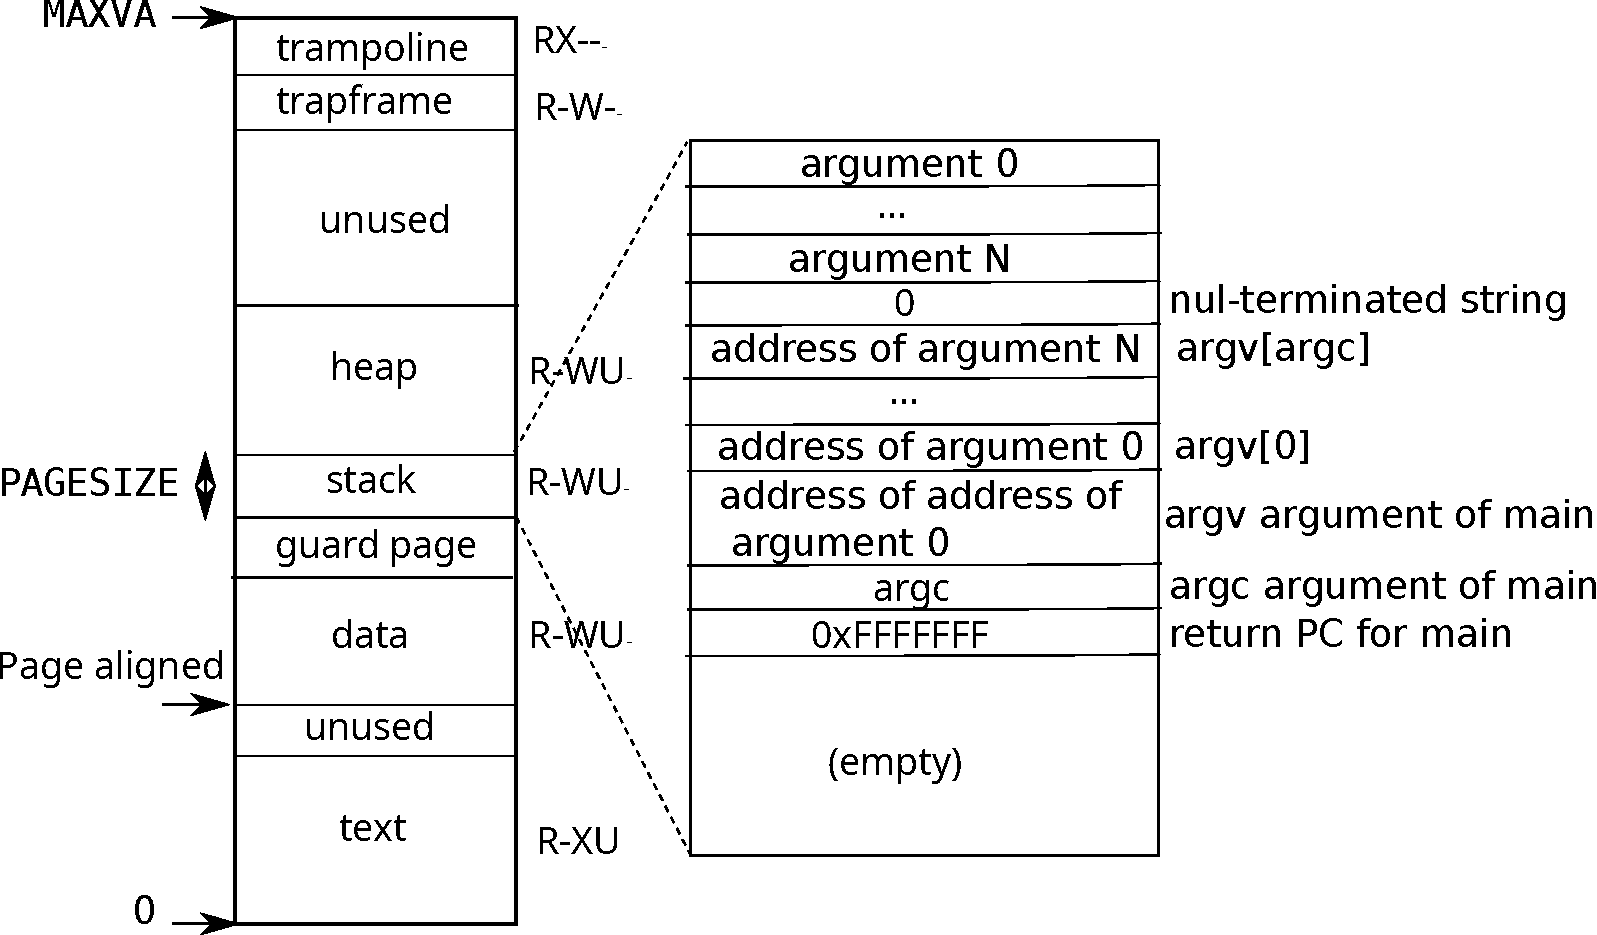
\includegraphics[scale=0.5]{fig/processlayout.pdf}
\caption{进程的用户地址空间及其初始堆栈。  }
\label{fig:processlayout}
\end{figure}     

   \section{代码:sbrk  }     

   \lstinline{sbrk}    是进程收缩或增加其内存的系统调用。系统调用是通过函数实现的
    \lstinline{growproc}   
    \lineref{kernel/proc.c:/^growproc/}    。
    \lstinline{growproc}    调用    \lstinline{uvmalloc}    或
    \lstinline{uvmdealloc}    ,取决于    \lstinline{n}    是正数还是负数。
    \lstinline{uvmalloc}   
    \lineref{kernel/vm.c:/^uvmalloc/}    使用  {    \tt    kalloc   }  分配物理内存,并使用  {    \tt    mappages   }  将 PTE 添加到用户页表中。
    \lstinline{uvmdealloc}    调用
  {    \tt    uvmunmap   } 
  \lineref{kernel/vm.c:/^uvmunmap/}   ,它使用  {    \tt    work   }  查找 PTE 和
  {    \tt    kfree   }  释放它们引用的物理内存。  

Xv6 使用进程的页表不仅告诉硬件如何映射用户虚拟地址,而且还作为将哪些物理内存页分配给该进程的唯一记录。这就是释放用户内存(在  {    \tt    uvmunmap   }  中)需要检查用户页表的原因。
    \section{代码:执行  }   
    \lstinline{exec}    是一个系统调用,它用从文件(称为二进制文件或可执行文件)读取的数据替换进程的用户地址空间。二进制文件通常是编译器和链接器的输出,并保存机器指令和程序数据。
    \lstinline{exec}       \lineref{kernel/exec.c:/^exec/}     使用    \indexcode{namei}    打开命名的二进制文件    \lstinline{path}   
    \lineref{kernel/exec.c:/namei/}   ,在 Chapter~    \ref{CH:FS}    中进行了解释。然后,它读取 ELF 标头。 Xv6 二进制文件采用广泛使用的    \indextext{ELF format}    格式,定义于
    \fileref{kernel/elf.h}    。 ELF 二进制文件由 ELF 标头组成,
    \indexcode{struct elfhdr}       \lineref{kernel/elf.h:/^struct.elfhdr/}    ,后跟一系列程序段标头,
    \lstinline{struct proghdr}       \lineref{kernel/elf.h:/^struct.proghdr/}   。每个
    \lstinline{progvhdr}    描述了必须加载到内存中的应用程序部分; xv6 程序有两个程序节头:一个用于指令,一个用于数据。  

第一步是快速检查该文件是否可能包含 ELF 二进制文件。 ELF 二进制文件以四字节“幻数”开头
    \lstinline{0x7F}    ,
    \lstinline{`E'}    ,
    \lstinline{`L'}    ,
    \lstinline{`F'}   ,或
    \indexcode{ELF_MAGIC}   
    \lineref{kernel/elf.h}{3}    。如果 ELF header 有正确的幻数,
    \lstinline{exec}    假定二进制文件格式良好。  

   \lstinline{exec}    分配一个没有用户映射的新页表
    \indexcode{proc_pagetable}   
    \lineref{kernel/exec.c:/proc_pagetable/}    ,为每个 ELF 段分配内存
    \indexcode{uvmalloc}   
    \lineref{kernel/exec.c:/uvmalloc/}    ,并将每个段加载到内存中
    \indexcode{loadseg}   
    \lineref{kernel/exec.c:/loadseg/}    。
    \lstinline{loadseg}    使用
    \indexcode{walkaddr}    查找要写入 ELF 段的每个页面的已分配内存的物理地址,以及
    \indexcode{readi}    从文件中读取。  

程序节标题为
    \indexcode{/init}   ,第一个用户程序创建
    \lstinline{exec}    ,看起来像这样:
    \begin{footnotesize}
\begin{verbatim}
# objdump -p user/_init

user/_init:     file format elf64-little

Program Header:
0x70000003 off    0x0000000000006bb0 vaddr 0x0000000000000000
                                       paddr 0x0000000000000000 align 2**0
         filesz 0x000000000000004a memsz 0x0000000000000000 flags r--
    LOAD off    0x0000000000001000 vaddr 0x0000000000000000
                                       paddr 0x0000000000000000 align 2**12
         filesz 0x0000000000001000 memsz 0x0000000000001000 flags r-x
    LOAD off    0x0000000000002000 vaddr 0x0000000000001000
                                       paddr 0x0000000000001000 align 2**12
         filesz 0x0000000000000010 memsz 0x0000000000000030 flags rw-
   STACK off    0x0000000000000000 vaddr 0x0000000000000000
                                       paddr 0x0000000000000000 align 2**4
         filesz 0x0000000000000000 memsz 0x0000000000000000 flags rw-
\end{verbatim}
\end{footnotesize}     

我们看到文本段应该从文件中偏移量 0x1000 处的内容加载到内存中的虚拟地址 0x0(没有写权限)。我们还看到数据应该加载到地址 0x1000,该地址位于页边界,并且没有可执行权限。  

程序节标题
    \lstinline{filesz}    可能小于
    \lstinline{memsz}    ,表示它们之间的间隙应该用零填充(对于 C 全局变量)而不是从文件中读取。为了
    \lstinline{/init}    ,数据
    \lstinline{filesz}    是 0x10 字节并且
    \lstinline{memsz}    是 0x30 字节,因此
    \indexcode{uvmalloc}    分配足够的物理内存来容纳 0x30 字节,但仅从文件中读取 0x10 字节
    \lstinline{/init}    。  

现在
    \indexcode{exec}    分配并初始化用户堆栈。它只分配一个堆栈页。
    \lstinline{exec}    将参数字符串一次复制到堆栈顶部,并将指向它们的指针记录在
    \indexcode{ustack}    。它将一个空指针放置在将要执行的内容的末尾
    \indexcode{argv}    列表传递到
    \lstinline{main}    。中的前三个条目
    \lstinline{ustack}    是假返回程序计数器,
    \indexcode{argc}    和
    \lstinline{argv}    指针。  

   \lstinline{exec}    在堆栈页正下方放置了一个不可访问的页,因此尝试使用多个页的程序将会出错。这个无法访问的页面还允许
    \lstinline{exec}    处理太大的参数;在这种情况下,
    \indexcode{copyout}   
    \lineref{kernel/vm.c:/^copyout/}    函数
    \lstinline{exec}    用于将参数复制到堆栈时会注意到目标页面不可访问,并将返回 -1。  

在准备新的内存映像期间,如果
    \lstinline{exec}    检测到错误,例如无效的程序段,它跳转到标签
    \lstinline{bad}    ,释放新图像,并返回-1。
    \lstinline{exec}    必须等待释放旧映像,直到确定系统调用将成功:如果旧映像消失,系统调用无法向其返回 -1。唯一的错误情况是
    \lstinline{exec}    在图像创建期间发生。图像完成后,
    \lstinline{exec}   可以提交到新页表
    \lineref{kernel/exec.c:/pagetable.=.pagetable/}    并释放旧的
    \lineref{kernel/exec.c:/proc_freepagetable/}    。  

   \lstinline{exec}    将 ELF 文件中的字节加载到内存中 ELF 文件指定的地址处。用户或进程可以将他们想要的任何地址放入 ELF 文件中。因此
    \lstinline{exec}    是有风险的,因为 ELF 文件中的地址可能无意或有意地引用内核。粗心的内核所造成的后果可能包括从崩溃到恶意破坏内核隔离机制(即安全漏洞)。 Xv6 执行许多检查来避免这些风险。例如
    \lstinline{if(ph.vaddr + ph.memsz < ph.vaddr)}    检查总和是否溢出 64 位整数。危险在于用户可以使用以下命令构建 ELF 二进制文件:
    \lstinline{ph.vaddr}    指向用户选择的地址,并且
    \lstinline{ph.memsz}    足够大,总和会溢出到 0x1000,这看起来像是有效值。在旧版本的 xv6 中,用户地址空间也包含内核(但在用户模式下不可读写),用户可以选择与内核内存相对应的地址,从而将数据从 ELF 二进制文件复制到内核中。在 xv6 的 RISC-V 版本中,这种情况不会发生,因为内核有自己独立的页表;
    \lstinline{loadseg}    加载到进程的页表中,而不是加载到内核的页表中。  

内核开发人员很容易忽略关键的检查,并且现实世界的内核长期以来一直缺少检查,用户程序可以利用这些检查的缺失来获取内核权限。 xv6 很可能没有完成验证提供给内核的用户级数据的完整工作,恶意用户程序可能能够利用这些数据来规避 xv6 的隔离。
    \section{真实世界  }     

与大多数操作系统一样,xv6 使用分页硬件进行内存保护和映射。大多数操作系统通过结合分页和页错误异常来比 xv6 更复杂地使用分页,我们将在第    \ref{CH:TRAP}    章中讨论这一点。  

Xv6 的简化是通过内核使用虚拟地址和物理地址之间的直接映射,并假设在地址 0x8000000 处存在物理 RAM,这是内核期望加载的位置。这适用于 QEMU,但在真实硬件上,事实证明这是一个坏主意;真实硬件将 RAM 和设备放置在不可预测的物理地址处,因此(例如)0x8000000 处可能没有 RAM,xv6 期望能够在此处存储核心。更严格的内核设计利用页表将任意硬件物理内存布局转换为可预测的内核虚拟地址布局。  

RISC-V支持物理地址级别的保护,但xv6没有使用该功能。  

在具有大量内存的计算机上,使用 RISC-V 对“超级页面”的支持可能很有意义。当物理内存较小时,小页面很有意义,以允许以细粒度分配和页出到磁盘。例如,如果一个程序仅使用 8 KB 内存,则为其提供整个 4 MB 物理内存超级页面是一种浪费。较大的页面对于具有大量 RAM 的机器来说是有意义的,并且可以减少页表操作的开销。  

xv6 内核缺少可以为小对象提供内存的类似  {    \tt    malloc   }  的分配器,从而阻止内核使用需要动态分配的复杂数据结构。更复杂的内核可能会分配许多不同大小的小块,而不是(如在 xv6 中)仅 4096 字节块;真正的内核分配器需要处理小分配和大分配。  

内存分配是一个长期的热门话题,基本问题是有效利用有限的内存并为未知的未来请求做好准备~    \cite{knuth}    。如今,人们更关心速度而不是空间效率。
    \section{练习  }     

   \begin{enumerate}

 
   \item   解析 RISC-V 的设备树以查找计算机拥有的物理内存量。   \item   编写一个用户程序,通过调用将其地址空间增加一个字节
    \lstinline{sbrk(1)}    。运行程序并在调用之前调查程序的页表
    \lstinline{sbrk}    和调用之后
    \lstinline{sbrk}    。内核分配了多少空间?新内存的 PTE 包含什么?   \item   修改 xv6 以对内核使用超级页面。   \item   Unix 实现
    \lstinline{exec}    传统上包括对 shell 脚本的特殊处理。如果要执行的文件以文本开头
    \lstinline{#!}    ,则第一行被视为要运行以解释文件的程序。例如,如果
 调用   \lstinline{exec}   运行
    \lstinline{myprog}   
    \lstinline{arg1}    和
    \lstinline{myprog}    的第一行是
    \lstinline{#!/interp}   ,那么
    \lstinline{exec}    运行
 带命令行的    \lstinline{/interp}   
    \lstinline{/interp}   
    \lstinline{myprog}   
    \lstinline{arg1}    。在 xv6 中实现对此约定的支持。   \item   为内核实现地址空间布局随机化。  \end{enumerate}     


